\documentclass[hyperref={pdfpagelabels=false},table]{beamer}
\usepackage{Estilo/slides-utfpr}

%\hypersetup{pdfpagemode=FullScreen}   %%% para deixar no modo de tela cheia
\beamertemplatenavigationsymbolsempty   %%% para não mostrar ícones de navegação
% no canto direito inferior

% Nome da disciplina - informação que somente aparece nas propriedades do arquivo PDF
\subject{Sistemas Distribuídos - UTFPR}

\title[Marcelo Gervazoni Carbonera]{Classificação de
caracteres (EMNIST) usando CNN}
\subtitle{Aprendizado de Máquina}
\author[Aprendizado de Máquina]{Marcelo Gervazoni Carbonera}{}
\institute[UTFPR]{ 
\small{\textbf{Universidade Tecnológica Federal do Paraná}}\\
Câmpus Pato Branco}

\date{12 de Julho de 2019}

%%%%%%%%%%%%%%%%%%%%%%%%%%%%%%%%%%%%%%%%%%%
%% Para usar subfiguras %%
%%%%%%%%%%%%%%%%%%%%%%%%%%%%%%%%%%%%%%%%%%%
%\usepackage{caption}
\usepackage{subcaption}

% Código python
\usepackage{pythonhighlight}

%% ============== \begin ====================
\begin{document}

\begin{frame}
	\titlepage
\end{frame}

\section{Classificação de caracteres (EMNIST) usando CNN}

\subsection{Base de Dados EMNIST}
\begin{frame}
	\frametitle{Base de Dados EMNIST}
	\begin{exampleblock}{Extended MNIST (Modified National Institute of Standards
	and Technology)}
		\begin{itemize}
		  \item Imagens de caracteres escritos à mão. 
		  \item 375974 imagens de 45x45 pixels (1 ou 0).
		  \item Distribuídas em 82 classes.
		\end{itemize}
	\end{exampleblock}
	\pause
	\begin{block}{Dados}
		\begin{itemize}
		  \item Imagens estão dispostas em pastas distintas para cada classe.
		  \item Classes: '!', '(', ')', '+', ',', '-', '0', '1', '2', '3', '4', '5',
		  '6', '7', '8', '9', '=', 'A', 'alpha', 'ascii\_124', 'b', 'beta', 'C',
		  'cos', 'd', 'Delta', 'div', 'e', 'exists', 'f', 'forall', 'forward\_slash',
		  'G', 'gamma', 'geq', 'gt', 'H', 'i', 'in', 'infty', 'int', 'j', 'k', 'l',
		  'lambda', 'ldots', 'leq', 'lim', 'log', 'lt', 'M', 'mu', 'N', 'neq', 'o',
		  'p', 'phi', 'pi', 'pm', 'prime', 'q', 'R', 'rightarrow', 'S', 'sigma',
		  'sin', 'sqrt', 'sum', 'T', 'tan', 'theta', 'times', 'u', 'v', 'w', 'X', 'y',
		  'z', '[', ']', '\{', '\}'
		\end{itemize}
	\end{block}
\end{frame}

\begin{frame}
	\frametitle{Classes desbalanceadas:}
	%\fbox{}
	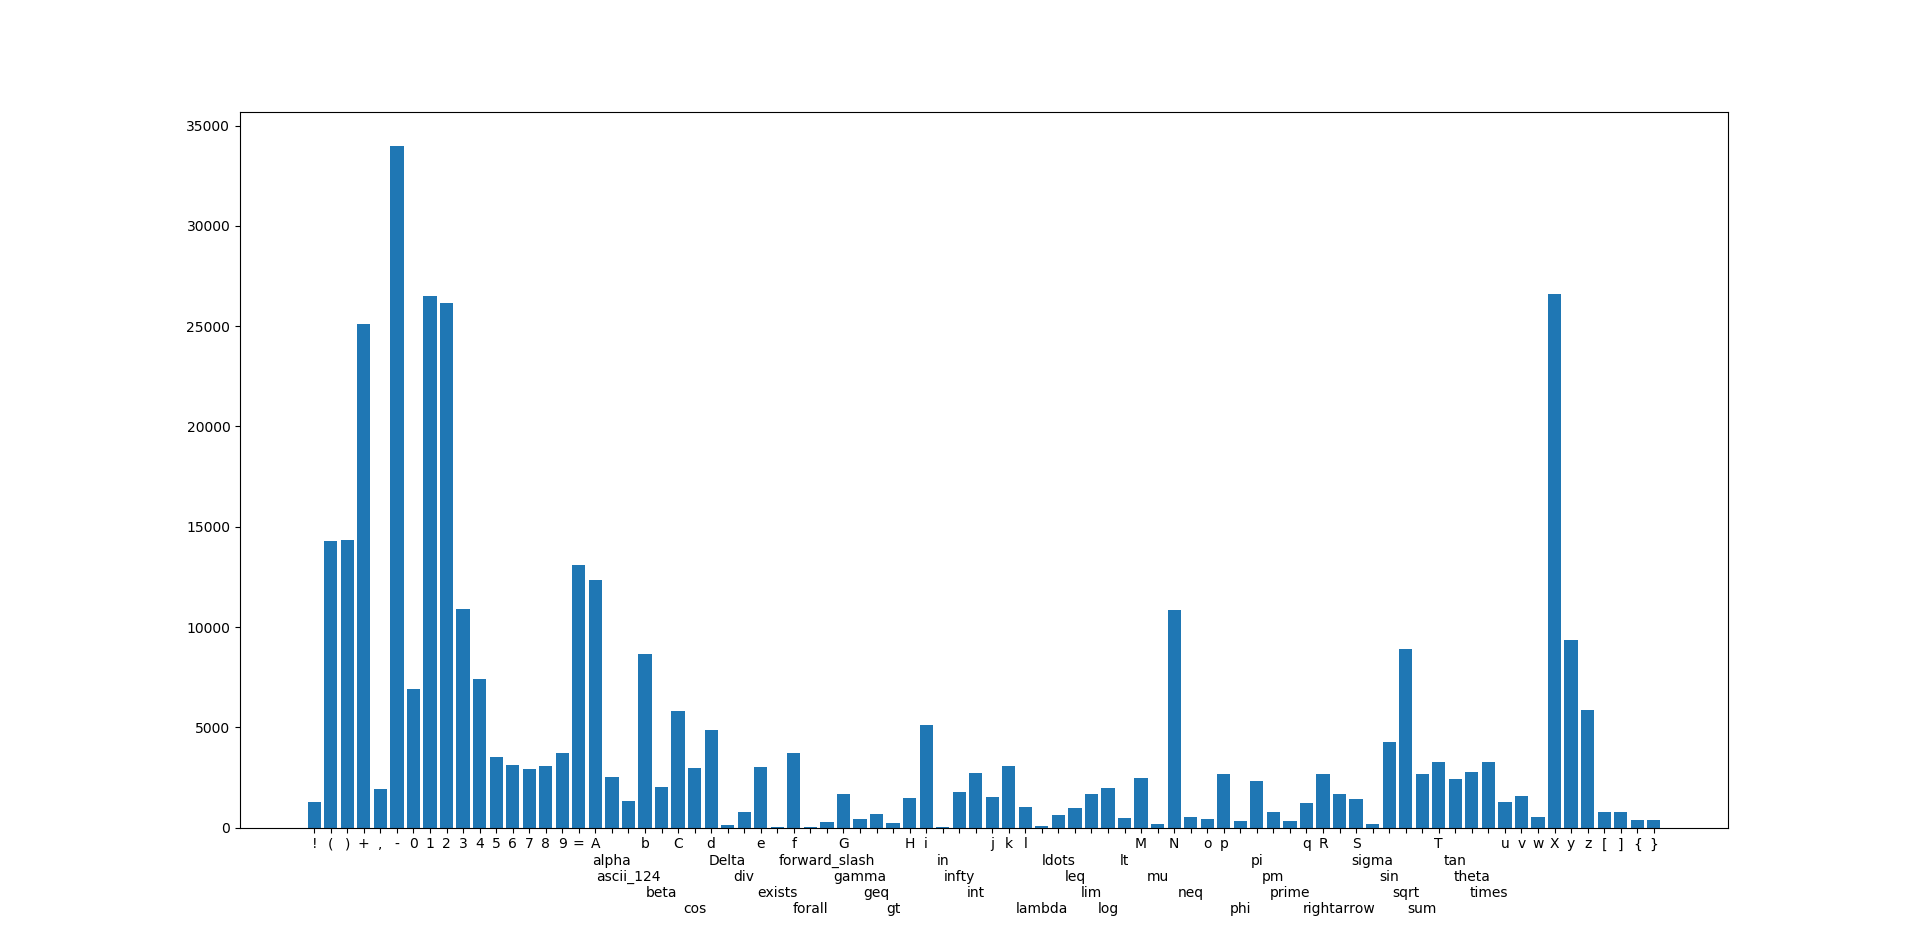
\includegraphics[scale = 0.305,trim = {5cm 0.5cm 5cm
	3cm}]{Figuras/Desbalanceado}
\end{frame}

\begin{frame}[containsverbatim]
	\frametitle{Código}
	\begin{exampleblock}{Codigos:}
		\begin{lstlisting}[language=python, showspaces=false, breaklines=true,
		keepspaces=true, numbers=left, numberfirstline=false]
import numpy as np
import os
import random as rd
from skimage import io, color

import keras
from keras.models import Sequential
from keras.layers import Dense, Dropout, Flatten
from keras.layers import Conv2D, MaxPooling2D
from keras.layers.convolutional import Convolution2D
		\end{lstlisting}
	\end{exampleblock}
\end{frame}

\begin{frame}[containsverbatim]
	\begin{exampleblock}{Códigos:}
		\begin{lstlisting}[language=python, showspaces=false, breaklines=true,
		keepspaces=true, numbers=left, numberfirstline=false]
## Porcentagem de treinamento:
tx_treinamento = 0.2

## Imprime nome das pastas
base = os.getcwd()
i = 0
VarDir = [];
for root, dirs, files in os.walk(os.getcwd(), topdown=False):
    for name in dirs:
        i=i+1
        VarDir.append(os.path.join(root, name))

# Extrair nomes das classes
k = VarDir.pop(82)
classes = []
for i in range(0, len(VarDir)):
    x = VarDir[i].split(os.sep)
    classes.append(x[-1])		
		\end{lstlisting}
	\end{exampleblock}
\end{frame}

\begin{frame}[containsverbatim]
	\begin{exampleblock}{Códigos:}
		\begin{lstlisting}[language=python, showspaces=false, breaklines=true,
		keepspaces=true, numbers=left, numberfirstline=false]
# Percorremos as pastas. Para cada uma, obter lista com nomes das imagens
SomaImagens = 0
x_treina = []
y_treina = []
x_teste = []
y_teste = []
# i caminha em diretórios (classes distintas)
numero_classes = len(VarDir)
#numero_classes = 2
for i in range(0, numero_classes): #len(VarDir)
    # Percorrendo arquivos na pasta:
    ListaArquivo = os.listdir(VarDir[i])
    
    # Soma de imagens carregadas
    SomaImagens = SomaImagens + len(ListaArquivo)
    print('Imagens carregadas:', SomaImagens)
    
    # Separar aleatoriamente imagens para treinamento e teste
    rd.shuffle(ListaArquivo)
		\end{lstlisting}
	\end{exampleblock}
\end{frame}

\begin{frame}[containsverbatim]
	\begin{exampleblock}{Códigos:}
		\begin{lstlisting}[language=python, showspaces=false, breaklines=true,
		keepspaces=true, numbers=left, numberfirstline=false]
	# Numero de linhas e colunas na primeira imagem:    
    Im = io.imread(VarDir[i] + '\\' + ListaArquivo[0])
    lin, col = Im.shape

    # j caminha sobre figuras nas pastas especificadas por i
    total_imagens_na_pasta = len(ListaArquivo)
    for j in range(0,total_imagens_na_pasta):
        # Abre figura
        Im = io.imread(VarDir[i] + '\\' + ListaArquivo[j])
        Im = color.rgb2gray(Im) > 127
	# Porcentagem treinamento ou teste
        if(j/total_imagens_na_pasta <= tx_treinamento): # Treinamento
            x_treina.append(Im)
            y_treina.append(i) # i é a classe
        else: # Teste
            x_teste.append(Im)
            y_teste.append(i) # i é a classe
		\end{lstlisting}
	\end{exampleblock}
\end{frame}

\begin{frame}[containsverbatim]
	\begin{exampleblock}{Códigos:}
		\begin{lstlisting}[language=python, showspaces=false, breaklines=true,
		keepspaces=true, numbers=left, numberfirstline=false]
x_treina = np.array(x_treina)
y_treina = np.array(y_treina)
x_teste = np.array(x_teste)
y_teste = np.array(y_teste)

################
# Etapa do CNN #
################
x_treina = x_treina.reshape(len(x_treina),45,45,1)
x_teste = x_teste.reshape(len(x_teste),45,45,1)

batch_size = 128
#num_classes = 10 #Variavel numero_classes
epochs = 20

print('x_treina shape:', x_treina.shape)
print(x_treina.shape[0], 'train samples')
print(x_teste.shape[0], 'test samples')
		\end{lstlisting}
	\end{exampleblock}
\end{frame}

\begin{frame}[containsverbatim]
	\begin{exampleblock}{Códigos:}
		\begin{lstlisting}[language=python, showspaces=false, breaklines=true,
		keepspaces=true, numbers=left, numberfirstline=false]
# convert class vectors to binary class matrices
y_treina = keras.utils.to_categorical(y_treina, numero_classes)
y_teste = keras.utils.to_categorical(y_teste, numero_classes)

model = Sequential()
model.add(Convolution2D(32, kernel_size=(3, 3),
                 activation='relu',
                 input_shape=(45,45,1)))
model.add(Convolution2D(64, (3, 3), activation='relu'))
model.add(MaxPooling2D(pool_size=(2, 2)))
model.add(Dropout(0.25))
model.add(Flatten())
model.add(Dense(128, activation='relu'))
model.add(Dropout(0.5))
model.add(Dense(numero_classes, activation='softmax'))

model.compile(loss=keras.losses.categorical_crossentropy,
              optimizer=keras.optimizers.Adadelta(),
              metrics=['accuracy'])
		\end{lstlisting}
	\end{exampleblock}
\end{frame}

\begin{frame}[containsverbatim]
	\begin{exampleblock}{Códigos:}
		\begin{lstlisting}[language=python, showspaces=false, breaklines=true,
		keepspaces=true, numbers=left, numberfirstline=false]
model.fit(x_treina, y_treina,
          batch_size=batch_size,
          epochs=epochs,
          verbose=1,
          validation_data=(x_teste, y_teste))
score = model.evaluate(x_teste, y_teste, verbose=0)
print('Test loss:', score[0])
print('Test accuracy:', score[1])

		\end{lstlisting}
	\end{exampleblock}
	\begin{block}{Salvar modelo:}
		\begin{lstlisting}[language=python, showspaces=false,
		breaklines=true,keepspaces=true, numbers=left, numberfirstline=false] model_json = model.to_json()
with open("model.json","w") as json_file:
	json_file.write(model_json)
model.save_weights("model.h5")
		\end{lstlisting}
	\end{block}
\end{frame}

\begin{frame}[containsverbatim]
	\begin{exampleblock}{Carregar modelo salvo:}
		\begin{lstlisting}[language=python, showspaces=false, breaklines=true,
		keepspaces=true, numbers=left, numberfirstline=false]
from keras.models import model_from_json

json_file = open('model.json', 'r')
loaded_model_json = json_file.read()
json_file.close()

loaded_model = model_from_json(loaded_model_json)
loaded_model.load_weights("model.h5")

print('Modelo importado.');
# Compilar modelo:
loaded_model.compile(loss=keras.losses.categorical_crossentropy, optimizer=keras.optimizers.Adadelta(),metrics=['accuracy'])
		\end{lstlisting}
	\end{exampleblock}
	\begin{block}{Resultado:}
		Test loss: 0.2169904357216396 \\
		Test accuracy: 0.9514195130511174
	\end{block}
\end{frame}

\begin{frame}
	\frametitle{Matriz de confusão:}
	\begin{figure}
		%\fbox{}
		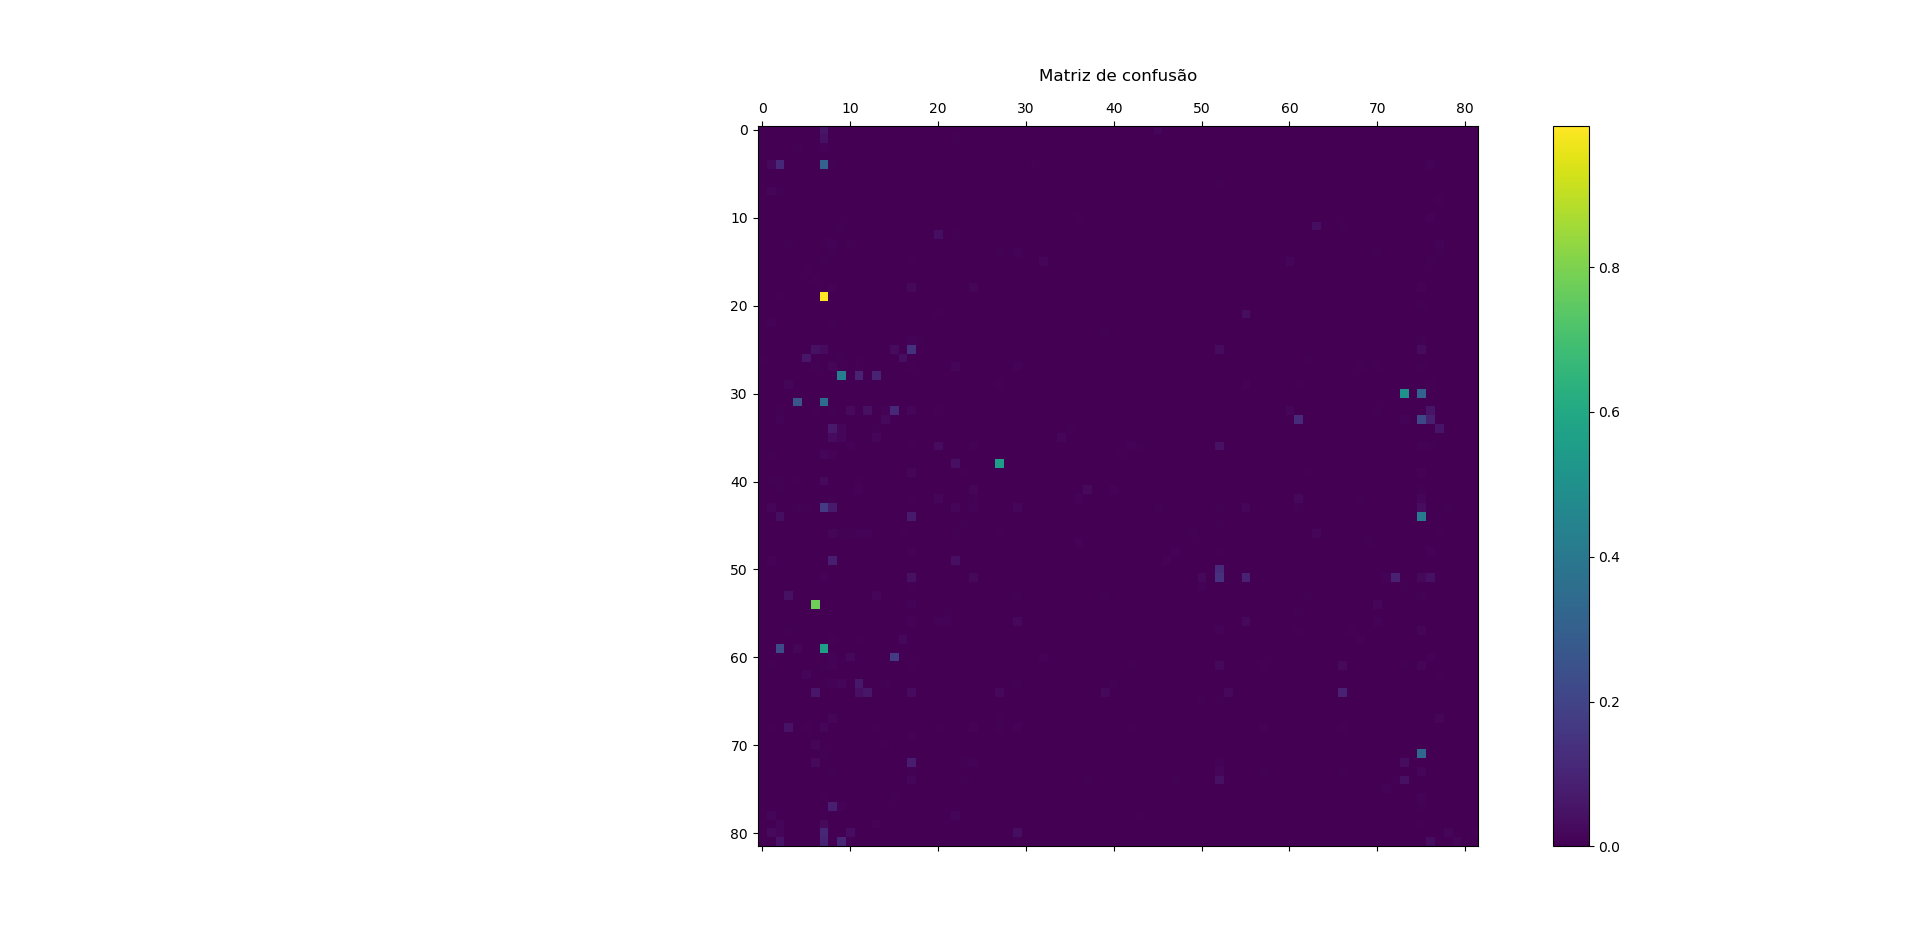
\includegraphics[scale = 0.38, trim ={18.5cm 1.5cm 7.5cm
		2cm}]{Figuras/Confusao}
	\end{figure}
\end{frame}

\begin{frame}
\begin{table}[]
\scalebox{0.65}{
\begin{tabular}{|l|l|l|l|l|l|}
\hline
DoGrupo        & Predição & Erro                 & NumdoGrupo & NumPredição & Razão                 \\ \hline
!              & 1        & 0.054615384615384614 & 1300       & 26520       & 0.049019607843137254  \\ \hline
,              & )        & 0.11647429171038824  & 1906       & 14355       & 0.13277603622431208   \\ \hline
,              & 1        & 0.3111227701993704   & 1906       & 26520       & 0.07187028657616892   \\ \hline
ascii\_124     & 1        & 0.9955190440627334   & 1339       & 26520       & 0.050490196078431374  \\ \hline
Delta          & A        & 0.145985401459854    & 137        & 12367       & 0.011077868521064122  \\ \hline
div            & -        & 0.06060606060606061  & 792        & 33997       & 0.023296173191752215  \\ \hline
exists         & 3        & 0.42857142857142855  & 21         & 10909       & 0.0019250160418003484 \\ \hline
exists         & 5        & 0.09523809523809523  & 21         & 3545        & 0.005923836389280677  \\ \hline
exists         & 7        & 0.09523809523809523  & 21         & 2909        & 0.007218975592987281  \\ \hline
forall         & v        & 0.5111111111111111   & 45         & 1558        & 0.028883183568677792  \\ \hline
forall         & X        & 0.3111111111111111   & 45         & 26594       & 0.0016921110024817629 \\ \hline
forward\_slash & ,        & 0.26181818181818184  & 275        & 1906        & 0.14428121720881426   \\ \hline
forward\_slash & 1        & 0.3527272727272727   & 275        & 26520       & 0.010369532428355957  \\ \hline
G              & 9        & 0.11229314420803782  & 1692       & 3737        & 0.45276960128445276   \\ \hline
G              & y        & 0.057919621749408984 & 1692       & 9340        & 0.18115631691648823   \\ \hline
gamma          & R        & 0.1198044009779951   & 409        & 2671        & 0.15312616997379258   \\ \hline
gamma          & X        & 0.21515892420537897  & 409        & 26594       & 0.015379408889223133  \\ \hline
gamma          & y        & 0.08801955990220049  & 409        & 9340        & 0.043790149892933616  \\ \hline
geq            & 2        & 0.06926406926406926  & 693        & 26141       & 0.026510079951034774  \\ \hline
geq            & z        & 0.05772005772005772  & 693        & 5870        & 0.11805792163543441   \\ \hline
in             & e        & 0.5531914893617021   & 47         & 3003        & 0.015651015651015652  \\ \hline
l              & 1        & 0.176007866273353    & 1017       & 26520       & 0.03834841628959276   \\ \hline
\end{tabular}}
\end{table}
\end{frame}

\begin{frame}
\begin{table}[]
\scalebox{0.65}{
\begin{tabular}{|l|l|l|l|l|l|}
\hline
DoGrupo        & Predição & Erro                 & NumdoGrupo & NumPredição & Razão                 \\ \hline
l              & 2        & 0.0727630285152409   & 1017       & 26141       &
0.03890440304502506   \\ \hline lambda         & A        & 0.07339449541284404  & 109        & 12367       & 0.008813778604350286  \\ \hline lambda         & X        & 0.41284403669724773  & 109        & 26594       & 0.004098668872678048  \\ \hline
lt             & 2        & 0.08176100628930817  & 477        & 26141       & 0.018247197888374585  \\ \hline
M              & N        & 0.11954765751211632  & 2476       & 10862       & 0.22795065365494385   \\ \hline
mu             & N        & 0.14124293785310735  & 177        & 10862       & 0.016295341557724177  \\ \hline
mu             & p        & 0.0903954802259887   & 177        & 2680        & 0.06604477611940299   \\ \hline
mu             & u        & 0.0903954802259887   & 177        & 1269        & 0.13947990543735225   \\ \hline
o              & 0        & 0.77728285077951     & 449        & 6914        & 0.06494070002892681   \\ \hline
prime          & )        & 0.23100303951367782  & 329        & 14355       & 0.02291884360849878   \\ \hline
prime          & 1        & 0.5623100303951368   & 329        & 26520       & 0.012405731523378581  \\ \hline
q              & 9        & 0.17479674796747968  & 1230       & 3737        & 0.32914102221032915   \\ \hline
S              & 5        & 0.06510969568294409  & 1413       & 3545        & 0.398589562764457     \\ \hline
sigma          & 0        & 0.05970149253731343  & 201        & 6914        & 0.0290714492334394    \\ \hline
sigma          & 6        & 0.05970149253731343  & 201        & 3118        & 0.06446440025657472   \\ \hline
sigma          & sqrt     & 0.08955223880597014  & 201        & 8908        & 0.022563987427031883  \\ \hline
times          & X        & 0.3343586588741926   & 3251       & 26594       & 0.12224561931262691   \\ \hline
u              & A        & 0.07880220646178093  & 1269       & 12367       & 0.10261178943963775   \\ \hline
z              & 2        & 0.08313458262350937  & 5870       & 26141       & 0.22455147086951532   \\ \hline
\{             & 1        & 0.10638297872340426  & 376        & 26520       & 0.014177978883861237  \\ \hline
\}             & 1        & 0.09549071618037135  & 377        & 26520       & 0.014215686274509804  \\ \hline
\}             & 3        & 0.10610079575596817  & 377        & 10909       & 0.03455862132184435   \\ \hline
\end{tabular}}
\end{table}
\end{frame}

%\begin{frame}[containsverbatim]
%	\begin{exampleblock}{Códigos:}
%		\begin{lstlisting}[language=python, showspaces=false, breaklines=true,
%		keepspaces=true, numbers=left, numberfirstline=false]
		
%		\end{lstlisting}
%	\end{exampleblock}
%\end{frame}

\begin{frame}
	\frametitle{Agradecimentos}
	\titlepage
\end{frame}

\end{document}